\chapter{Examples}
\label{chp:ex}

\begin{figure}[tp]
	\caption[Example]{Example}
	\centering
	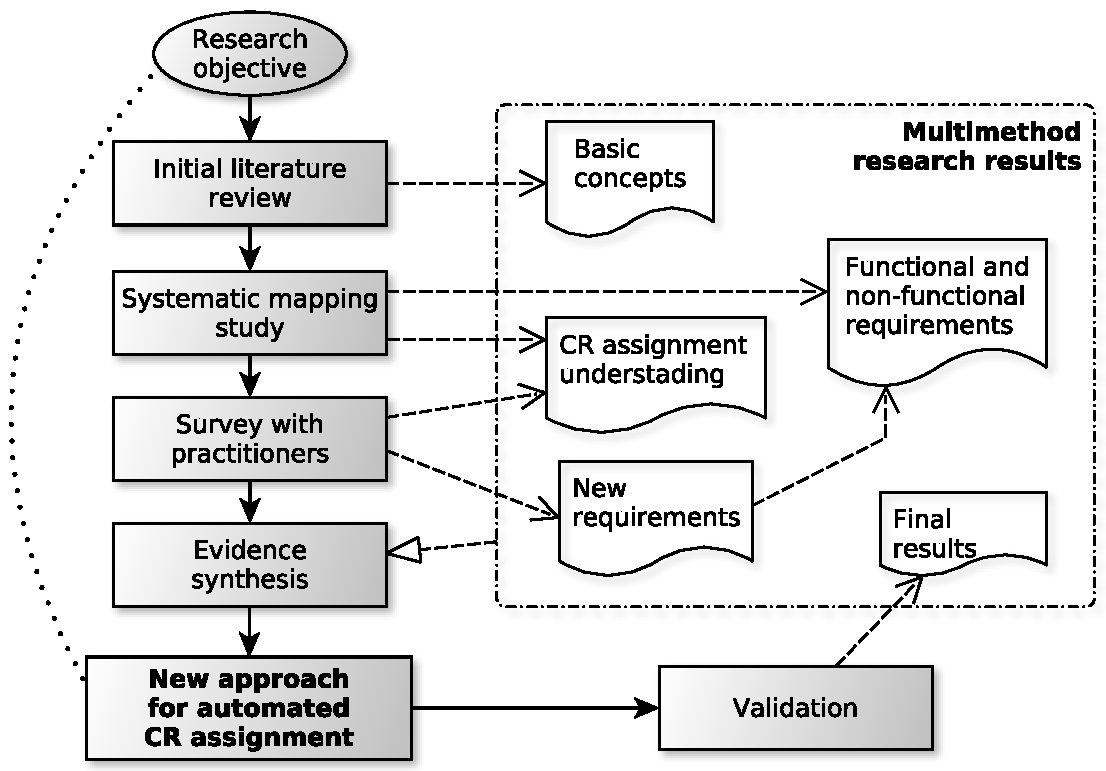
\includegraphics[width=0.75\columnwidth]{images/img1.pdf}
	\caption*{Fonte: \citep{einstein1907252}}
	\label{fig:graphexample}
\end{figure}

\begin{table}[bh]
	\centering
	\caption{Resumo dos operadores apresentados}
	\label{tbl:resumo_operadores}
	\begin{tabularx}{\linewidth}{|X|X|X|}
		\hline
		\textbf{Operador} & \textbf{Operação} & \textbf{Referência} \\
		\hline
		\textit{Random Centering} & Criação de Indivíduos & Proposto neste trabalho \\
		\hline
		\textit{Approximated Maximum Distance Centering} & Criação de Indivíduos & Proposto neste trabalho \\
		\hline
		\textit{Random Partitioning} & Criação de Indivíduos & Proposto neste trabalho \\
		\hline
		\textit{Heuristic Graph Partitioning} & Criação de Indivíduos & Proposto neste trabalho \\
		\hline
		\textit{Random Path Building} & Criação de Indivíduos & Proposto neste trabalho \\
		\hline
		\textit{Nearest Neighbor Path Building} & Criação de Indivíduos & EXAMPLE \\
		\hline
		\textit{Nearest Insertion Path Building} & Criação de Indivíduos & EXAMPLE \\
		\hline
		Melhorar & Mutação & Proposto neste trabalho \\
		\hline
		\textit{2-change} & Mutação & EXAMPLE \\
		\hline
		\textit{Half Add Half Sub Small Changes} & Mutação & Proposto neste trabalho \\
		\hline
		\textit{Half Add Half Sub Rebuild} & Mutação & Proposto neste trabalho \\
		\hline
		\textit{Simple Random Crossover} & Recombinação & Proposto neste trabalho \\
		\hline
	\end{tabularx}
	\caption*{Fonte: O autor}
\end{table}


\begin{algorithm}                  % enter the algorithm environment
	\caption{\textit{Heuristic Graph Partitioning}}          % give the algorithm a caption
	\label{partitioning_fungal}                           % and a label for \ref{} commands later in the document
	\algcomment{\begin{center} Fonte: O Autor \end{center}}
	\begin{algorithmic}[1]                    % enter the algorithmic environment
		\Procedure{GRAPH-PARTITIONING}{$centros, G(V,E)$}
		\newline
		\Comment{$G$ é o o grafo e $centros$ é a lista de centros calculados anteriormente}
		\State $ParticaoPorVertice \gets $ \{\}
		\State $ListaDeVerticesPorCentro \gets $ \{\}
		\State $ParticaoDoCentro \gets $ \{\}
		\For{$i \in V$}
			\If{$i \in centros$}
				\State $ParticaoPorVertice[i] \gets i$
			\Else
				\State $ParticaoPorVertice[i] \gets -1$
			\EndIf
		\EndFor
		\For{$centro \in centros$}
			\State $ListaDeVerticesPorCentro(centro) \gets $ lista dos nós do grafo ordenados pelas suas distâncias ao $centro$
			\State $ParticaoDoCentro(centro) \gets $ \{\}
		\EndFor
		\Repeat
			\For{$C_{i} \in centros$}
				\While{$ListaDeVerticesPorCentro(C_{i}) \neq \{\}$}
					\State $n \gets $ REMOVE-PRIMEIRO($ListaDeVerticesPorCentro(C_{i})$)
					\If{$ParticaoPorVertice(n) = -1$}
						\State $ParticaoPorVertice(n) \gets C_{i}$
						\State \textbf{Pare o Laço Enquanto}
					\EndIf
				\EndWhile
			\EndFor
		\Until{$-1 \notin ParticaoPorVertice$} \Comment{Até que todo vértice esteja em uma partição}
		\For{$v \in V$}
			\State $ParticaoDoCentro(ParticaoPorVertice(v)) \cup $ {o menor caminho entre ParticaoPorVertice(v) e v}
		\EndFor
		\State \textbf{Retorne} as partições em $ParticaoDoCentro$
		\EndProcedure
	\end{algorithmic}
\end{algorithm}

\tikzstyle{vertex}=[circle,fill=black!25,minimum size=20pt,inner sep=0pt]
\tikzstyle{red vertex}=[circle,fill=red!25,minimum size=20pt,inner sep=0pt]
\tikzstyle{green vertex}=[circle,fill=green!25,minimum size=20pt,inner sep=0pt]
\tikzstyle{green edge} = [draw,line width=2pt,-,green!50]
\tikzstyle{red edge} = [draw,line width=2pt,-,red!50]

\begin{figure}
	\caption{Exemplo de solução da \ac{tmap}}
	\centering
	\begin{tikzpicture}
	[scale=.8,auto=left,every node/.style={circle,fill=blue!20}]
	\node[vertex] (n6) at (1,6)  {6};
	\node[vertex] (n0) at (4,12) {0};
	\node[vertex] (n1) at (8,12) {1};
	\node[vertex] (n2) at (12,6) {2};
	\node[vertex] (n4) at (2,1)  {4};
	\node[red vertex] (n5) at (5,9)  {5};
	\node[vertex] (n7) at (10,1) {7};
	\node[green vertex] (n3) at (7,9)  {3};
	
	\foreach \from/\to in {n0/n6,n6/n4,n4/n5,n5/n0}
		\path[red edge] (\from) -- (\to);
	\foreach \source/\dest in {n1/n2,n2/n7,n7/n3,n3/n1}
		\path[green edge] (\source) -- (\dest);
	\foreach \de/\para in {n0/n1}
		\draw (\de) -- (\para);
	
	\end{tikzpicture}
	\caption*{Fonte: O autor}
	\label{fig:tmap_example}
\end{figure}
